\documentclass[nynorsk,journal,biblatex]{mnt}

\usepackage{graphicx}   % to import PNG, JPEG and PDF graphics

\journal{\emph{Nordic Journal of STEM Education}}
\doi{TBA} % This is required for journal, otherwise ignored
\Jvolume{4}
\Jnumber{2}
\firstpage{31} % Starting page number

\title{\LaTeX\ til \emph{Nordic Journal of STEM Education}}
\author{Hans Georg Schaathun,
\emph{NTNU --- Noregs Teknisk-Naturvitskaplege Universitet}}

\addbibresource{template.bib}


\begin{document}
\maketitle

\begin{abstract}
   Dette er eit døme på bruken av \texttt{mnt}-klassa for
   \LaTeX, slik ho vert brukt for \emph{Nordic Journal of STEM Education}.
\end{abstract}

\section{Innleiing}

Klassa vert brukt både til MNT-konferansen og til
\emph{Nordic Journal of STEM Education}.

Klassa bruker babel, og \emph{må} ha ein språkopsjon til
\verb|\documentclass|, typisk \texttt{nynorsk} eller \texttt{british}.

Opsjonen \texttt{journal} skal brukast for tidsskriftartiklar, 
men ikkje for konferanseartiklar.
Dette dømet bruker ogso opsjonen \texttt{biblatex}, som bruker
biblatex i staden for natbib.  Dette oppsettet krev kompilering
med biber og lualatex i staden for bibtex og pdflatex.  Sjå 
\texttt{Maketitle} for detaljar.

\begin{table}
\centering
  \caption{Karakterfordeling.}
  \begin{tabular}{l|r|r|r|r|r|r|}
     & \multicolumn{1}{c|}{A}
     & \multicolumn{1}{c|}{B}
     & \multicolumn{1}{c|}{C}
     & \multicolumn{1}{c|}{D}
     & \multicolumn{1}{c|}{E}
     & \multicolumn{1}{c|}{F} \\
  \hline
  2018 & 1 & 7 & 28 & 24 & 29 & 49 \\
  \hline
  2018 &
  \num{0.72}\% &
  \num{5.1}\% &
  \num{20.3}\% &
  \num{17.4}\% &
  \num{21.0}\% &
  \num{35.5}\%  \\
  \hline
  2017 &
  \num{1.5}\% &
  \num{5.1}\% &
  \num{15.4}\% &
  \num{14.7}\% &
  \num{20.6}\% &
  \num{42.6}\% \\
  \hline
  \end{tabular}
  \label{tab:grade}
\end{table}


Tabell~\ref{tab:grade} viser eit døme på tabell.

\begin{figure}
\begin{center}
  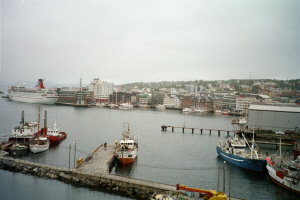
\includegraphics[width=0.6\textwidth]{tromso}
\end{center}
  \caption{Overblikk over Tromsø; teke frå broen mot Tromsdalen.
    Gustav Foseid (User:Gustavf on en.wikipedia)
    Juli 2003.
    Lisensiert under \emph{GNU Free Documentation License}.
    }
  \label{fig}
\end{figure}

Eit par andre døme:
\begin{itemize}
  \item 
Korte evalueringsspørsmål i førelesingane gjennom eit
      quizverkty \citep{hgs2018udit}.
   \begin{itemize}
     \item nøsting er lov
     \item ... men er det riktig kulesymbol?  Det må redaktøren svara på.
   \end{itemize}
  \item 
Figur~\ref{fig} viser Tromsø, der neste MNT-konferanse vert arrangert.
\end{itemize}

... og nummererte lister ...
\begin{enumerate}
  \item 
    \citet{biggs11a} sa at ...
  \item Punkt 2.
\end{enumerate}

Somme tider treng me sitat, t.d.\
\begin{quote}
Høge stryktal i matematikk er ei velkjend utfordring frå mange studium.
Emne- og studieansvarlege landet over freistar 
stadig nye tiltak for å auka gjennomstrauminga.
Matematikken er prega av sterke tradisjonar og forventingar om kva
studentane bør kunne.

\raggedleft\emph{Anonym matematikklærar}
\end{quote}
eller 
\begin{quotation}
Høge stryktal i matematikk er ei velkjend utfordring frå mange studium.
Emne- og studieansvarlege landet over freistar 
stadig nye tiltak for å auka gjennomstrauminga.
Matematikken er prega av sterke tradisjonar og forventingar om kva
studentane bør kunne.

Sitatet kan gjerne ha fleire avsnitt.

\raggedleft\emph{Anonym matematikklærar}
\end{quotation}
Bruk \verb.quotation. når sitatet har meir enn eitt avsnitt, og 
\verb.quote. når det anten er eitt avsnitt eller ein serie med 
einskildliner.
\LaTeX-stilen har vore kritisert for overdriven luft rundt sitat.
Me eksperimenterer difor med å bruka \verb.quoting. i staden.
\begin{quoting}
Høge stryktal i matematikk er ei velkjend utfordring frå mange studium.
Emne- og studieansvarlege landet over freistar 
stadig nye tiltak for å auka gjennomstrauminga.
Matematikken er prega av sterke tradisjonar og forventingar om kva
studentane bør kunne.

Sitatet kan gjerne ha fleire avsnitt.

\raggedleft\emph{Anonym matematikklærar}
\end{quoting}
Me kan godt diskutera kva som er best.

\section{Referanseliste}

Denne referansen har registrert DOI: \citet{ss2008cocreation}



% \bibliographystyle{plainnat}
% \bibliography{template}
\printbibliography

\end{document}
